\documentclass[12pt]{article}
\usepackage[margin=1in]{geometry}
\usepackage{setspace}
\usepackage{amsmath, amssymb}
\usepackage{booktabs}
\usepackage{graphicx}
\usepackage{caption}
\usepackage[round]{natbib}
\usepackage{hyperref}
\doublespacing
\graphicspath{{../../figures/}}

\title{A Neuro-Symbolic Search Pipeline for Binary Linear Systems:\\
LP-Guided Monte Carlo Tree Search with Null-Space Projection and\\
Policy-Guided Complete Backtracking}
\author{neuroMCTS project}
\date{July 2026}

\begin{document}
\maketitle

\begin{abstract}
Binary linear systems (BLS) arise in laser-based nondestructive testing, where a binary image must be reconstructed from integer-valued measurements and where noise may render the system unsatisfiable. Reliable feasibility detection and exact solution recovery are therefore both required at inference time. In this report, a neuro-symbolic pipeline is presented in which a bipartite graph neural network trained by AlphaZero-style Monte Carlo tree search is combined with three symbolic components: constraint propagation, an alternating-projection heuristic that walks along the null space of the coefficient matrix (kernel pump), and a policy-guided complete backtracking search with a node budget. On a held-out test set of 1{,}000 instances of size $10 \times 25$ (800 feasible, 200 infeasible), the pipeline attains 99.50\% feasibility-classification accuracy with zero false negatives and recovers exact solutions for 99.62\% of the feasible instances, exceeding all inexact baselines (LP relaxation rounding, LLL, BKZ) by 4.7--36.2 percentage points on feasibility and by 40.9--45.5 percentage points on solution accuracy. Exact solvers (Gurobi, SCIP, CP-SAT) remain perfect and faster at this instance size; the operational value of the proposed pipeline is therefore positioned in its anytime behavior and its learned components, whose scaling to larger systems is left to future work. An ablation of the decision stages shows that 61.1\% of test instances are closed by purely symbolic rules or the kernel pump before any neural inference, while the learned policy contributes through search on the remaining hard residue.
\end{abstract}

\section{Introduction}

Laser-based nondestructive testing reconstructs a binary object image from a set of linear measurements. When the scan is clean, a unique binary solution exists; when dust or measurement noise corrupts the target vector, no binary solution exists at all. The operational task is therefore twofold: (i) decide quickly whether the acquired system is consistent, so that a corrupted scan can be re-acquired instead of silently mis-reconstructed, and (ii) recover the exact binary image when the system is consistent. Both decisions must be made within an inference-time budget compatible with an inline inspection process.

Formally, given $A \in \{0,1\}^{m \times n}$ and $\mathbf{b} \in \mathbb{Z}^m$, a vector $\mathbf{x}^\ast \in \{0,1\}^n$ with $A\mathbf{x}^\ast = \mathbf{b}$ is sought, or a certificate that none exists. This feasibility problem is a market-split-type binary Diophantine system \citep{cornuejols1998market, aardal2000market}, and deciding feasibility is NP-complete in general. Lattice-based reformulations that exploit the null space of $A$ have historically been the most effective classical approach on such systems \citep{aardal2000market}, while LP-based branch-and-bound degrades rapidly as the number of equations grows.

In this report, the v5 iteration of the neuroMCTS pipeline is documented. The contribution of this iteration is threefold. First, the reinforcement-learning component was aligned with the AlphaZero recipe: the policy network is now trained against the full MCTS visit distribution rather than a single sampled action, and Dirichlet noise is injected at the search root during self-play only. Second, the null-space structure emphasized in the project formulation is operationalized as a \emph{kernel pump}: an alternating projection between the hypercube rounding and the affine solution subspace $\{\mathbf{x} : A\mathbf{x} = \mathbf{b}\}$, whose fixed points are constructive feasibility certificates. Third, the inference pipeline is completed by a \emph{policy-guided depth-first search} (DFS) with a node budget, which turns the learned variable and value orderings into either an exact solution or a proof of infeasibility on the residue of instances that defeat both the pump and the MCTS search.

\section{Problem Setting and Data}

Each instance consists of a dense binary coefficient matrix $A \in \{0,1\}^{10 \times 25}$ (density $\approx 0.5$) and a target vector $\mathbf{b} \in \mathbb{Z}^{10}$. The training set contains 10{,}000 instances (8{,}000 feasible, 2{,}000 infeasible); the test set contains 1{,}000 instances (800 feasible, 200 infeasible) and was never used for training, threshold calibration, or checkpoint selection. Feasible instances carry a ground-truth binary solution; infeasible instances model noise-corrupted scans.

Two evaluation metrics are reported, following the baseline harness: feasibility-classification accuracy over all instances (with the false-negative rate of particular operational interest, since a false negative discards a recoverable scan), and solution accuracy over the ground-truth-feasible instances, where a prediction counts only if $A\mathbf{x} = \mathbf{b}$ holds exactly. Reported per-instance times include LP relaxation, pseudo-inverse, and graph-construction preprocessing.

\section{Method}

\subsection{Learned components}

The network is a bipartite graph neural network over variable and constraint nodes with GAT message passing, LSTM node updates, and four heads: variable selection, value assignment, state value, and instance feasibility. The LP relaxation solution is attached to every variable node as a feature, and a residual-bucket status is attached to every constraint node. The network is pre-trained by masked-solution prediction on feasible instances and then trained by MCTS self-play. Three changes were introduced in v5. (i) The policy loss is the cross-entropy between the network's masked selection distribution and the full MCTS visit distribution, replacing a single-action REINFORCE-style loss; the assignment head is likewise trained against the visit-derived action distribution. (ii) Dirichlet noise ($\alpha = 0.3$, $\varepsilon = 0.25$) is mixed into the root priors during training only. (iii) Training-loop defects were repaired (learning-rate restoration after pre-training, per-epoch reset of the novelty-bonus table, history preservation across phases).

\subsection{Symbolic components}

\paragraph{Constraint propagation and probing.} Forced assignments are propagated to a fixed point; one-step probing detects variables whose assignment in either polarity yields a contradiction. A contradiction at the root is a proof of infeasibility.

\paragraph{Kernel pump.} Let $A^{+}$ denote the Moore--Penrose pseudo-inverse of $A$. Starting from the LP solution $\mathbf{x}_{\mathrm{LP}}$, the pump alternates $\mathbf{x}_r \leftarrow \mathrm{round}(\mathrm{clip}(\mathbf{x}))$ and $\mathbf{x} \leftarrow \mathbf{x}_r - A^{+}(A\mathbf{x}_r - \mathbf{b})$; the second step is an orthogonal projection onto the affine subspace $\{\mathbf{x} : A\mathbf{x}=\mathbf{b}\}$, i.e., a move along the null space of $A$. If a rounding step ever satisfies $A\mathbf{x}_r = \mathbf{b}$ exactly, a binary solution has been found and feasibility is certified constructively; cycling is broken by random partial reflips. The pump never mislabels an infeasible instance, since its only positive output is an exact solution. Within the full pipeline it closes 463 of the 800 feasible test instances; measured in isolation on a 100-instance sample, one pump invocation averaged 0.78\,ms.

\paragraph{Policy-guided complete backtracking.} When both the pump and the MCTS search fail, a depth-first backtracking search is run from the propagated root with variable order given by the selection head's logits and value order given by the assignment head, under a node budget of 20{,}000 propagated nodes. Exhausting the tree without a solution is a proof of infeasibility; exhausting the budget leaves the decision to the feasibility head. This stage generalizes the 1-ply backtracking used during MCTS rollouts into a complete search whose ordering is the learned policy, in the spirit of learned branching rules for exact solvers \citep{gasse2019exact}.

\subsection{Inference pipeline}

Each instance passes through: (1) propagation/probing (root contradiction $\Rightarrow$ infeasible); (2) the LP hard rule (LP infeasibility $\Rightarrow$ binary infeasibility); (3) the kernel pump (success $\Rightarrow$ solved); (4) the feasibility head at threshold $0.5$; (5) MCTS with 1-ply backtracking, followed by one pump-repair attempt from the terminal point; and (6) the policy-guided DFS. The threshold was calibrated on 1{,}000 training-set instances; the sweep showed no operating point better than $0.5$. The checkpoint (epoch 10 of 50) was chosen by the calibration set's ranking of the first and last checkpoints (75.25\% vs.\ 72.75\% solution accuracy); the per-checkpoint test-set numbers in Section~4.1 are reported post hoc for transparency and were not used for selection, though it is acknowledged that calibration scores for the intermediate checkpoints were not collected.

\section{Experiments}

\subsection{Training behavior}

The model was warm-started from the v4 pre-trained weights and trained for 50 self-play epochs (512 instances per epoch, 100 simulations per move). Training solved-rate stabilized near 0.70 by epoch 3, suffered a transient collapse to 0.30 at epoch 20 with full recovery by epoch 22, and fluctuated in the 0.63--0.69 band thereafter (Figure~\ref{fig:curve}). Test-set solution accuracy of the pipeline \emph{without} the DFS stage was highest at the epoch-10 checkpoint (76.12\%) and declined to 73.4--73.5\% at later checkpoints even as training metrics recovered, indicating instance memorization on the fixed 10{,}000-instance training pool. The calibration set reproduced the ranking of the first and last checkpoints (75.25\% at epoch 10 vs.\ 72.75\% at epoch 50), so the epoch-10 checkpoint was selected without consulting the test set; intermediate checkpoints were not scored on the calibration set (Section~3.3).

\begin{figure}[t]
\centering
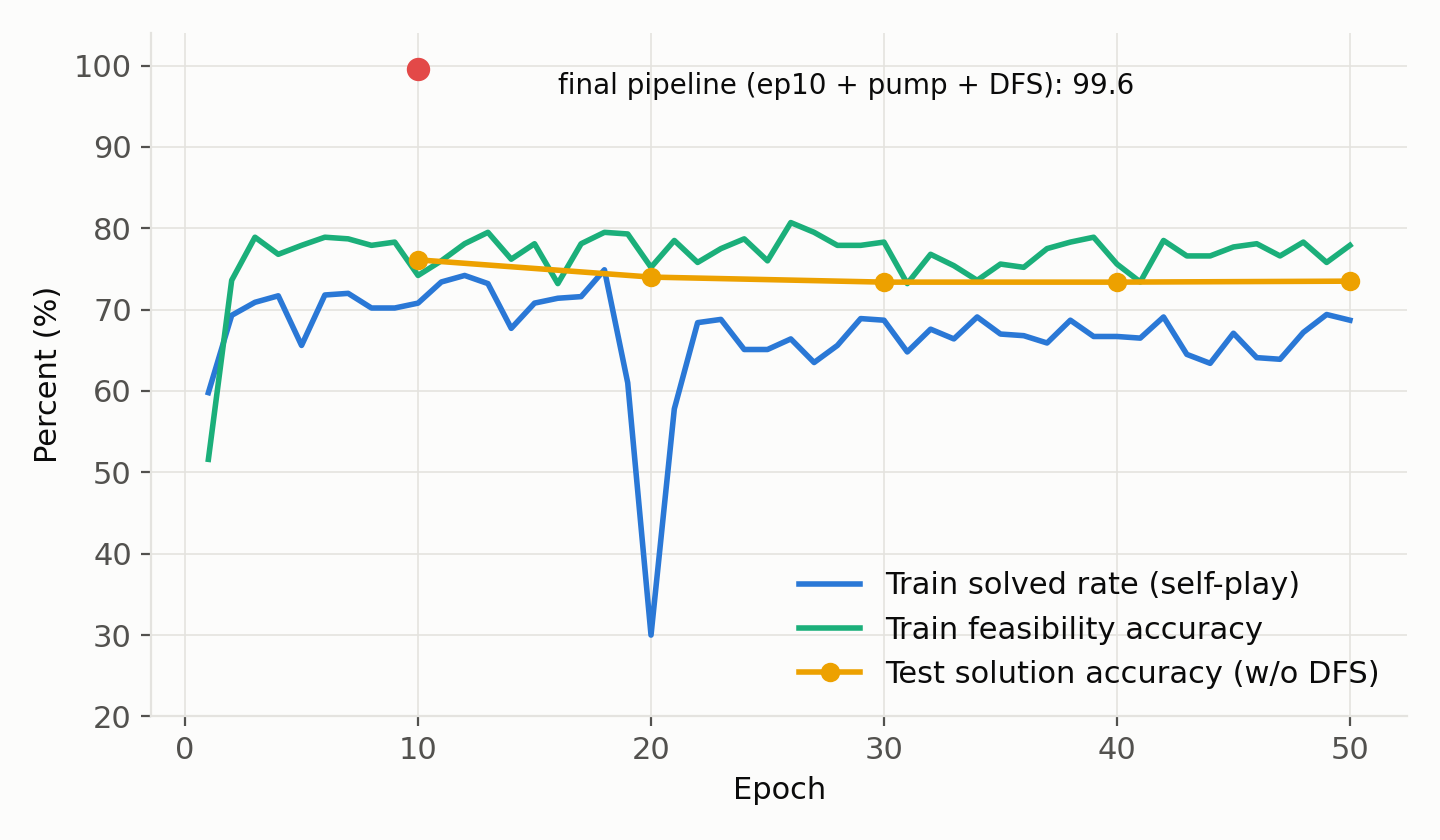
\includegraphics[width=0.9\textwidth]{v5_training_test_curve.png}
\caption{Self-play training metrics (per epoch) and test solution accuracy of the pipeline without the DFS stage, evaluated at every tenth checkpoint. The final pipeline point includes the kernel pump and policy-guided DFS.}
\label{fig:curve}
\end{figure}

\subsection{Main results}

Table~\ref{tab:main} compares the full pipeline against the seven project baselines on the 1{,}000-instance test set. The proposed pipeline reaches 99.50\% feasibility accuracy (zero false negatives; five false positives, all budget-exhausted DFS cases) and 99.62\% solution accuracy (797/800).

\begin{table}[t]
\centering
\caption{Test-set results ($10 \times 25$, 1{,}000 instances). Solution accuracy is over the 800 feasible instances. Baseline times exclude model/problem construction where the respective harnesses do so; the proposed method's time includes all preprocessing.}
\label{tab:main}
\begin{tabular}{lccc}
\toprule
Method & Feasibility acc.\ (\%) & Solution acc.\ (\%) & Avg.\ time (s) \\
\midrule
Gurobi MILP & 100.00 & 100.00 & 0.0022 \\
SCIP MILP & 100.00 & 100.00 & 0.0037 \\
CP-SAT (OR-Tools) & 100.00 & 100.00 & 0.0011 \\
LP relaxation + rounding (Gurobi) & 94.80 & 58.75 & 0.0005 \\
LP relaxation + rounding (SCIP) & 94.80 & 54.87 & 0.0016 \\
LLL (fpylll) & 63.30 & 54.12 & 0.0006 \\
BKZ (fpylll) & 63.40 & 54.25 & 0.0009 \\
\midrule
Proposed (v5, ep10 + pump + DFS) & 99.50 & 99.62 & 1.03 \\
\bottomrule
\end{tabular}
\end{table}

Two comparisons must be read separately. Against the inexact baselines that share the pipeline's anytime character, the proposed method dominates on both quality metrics: $+4.7$ points of feasibility accuracy and $+40.9$ points of solution accuracy over the strongest of them (Gurobi LP rounding), and roughly $+36$ points of feasibility accuracy over the lattice heuristics, whose feasibility errors are concentrated in false negatives (LLL/BKZ declare 366--367 recoverable scans infeasible). Against the exact solvers, the proposed pipeline is strictly worse at this instance size: Gurobi, SCIP, and CP-SAT are perfect and roughly 300--900 times faster (two to three orders of magnitude). No claim of superiority over exact solvers is made at $10 \times 25$; the case for the learned pipeline rests on inference-time scaling properties that remain to be demonstrated on larger systems.

\subsection{Stage attribution}

Figure~\ref{fig:breakdown} attributes each test instance to the stage that closed it. Purely symbolic rules close 148 infeasible instances (13 by propagation, 135 by the LP hard rule), and the kernel pump closes 463 feasible instances---together 61.1\% of the test set before any neural inference. The learned components close most of the remainder: MCTS solves 128 instances directly, pump repair adds 12, and the policy-guided DFS solves a further 194 and proves infeasibility of 47. Five infeasible instances exhaust the DFS budget and are misclassified as feasible; three feasible instances remain unsolved. (In the harness's stage labels these eight budget-exhausted instances are tallied under the MCTS bucket, which therefore counts $128 + 5 + 3 = 136$.)

\begin{figure}[t]
\centering
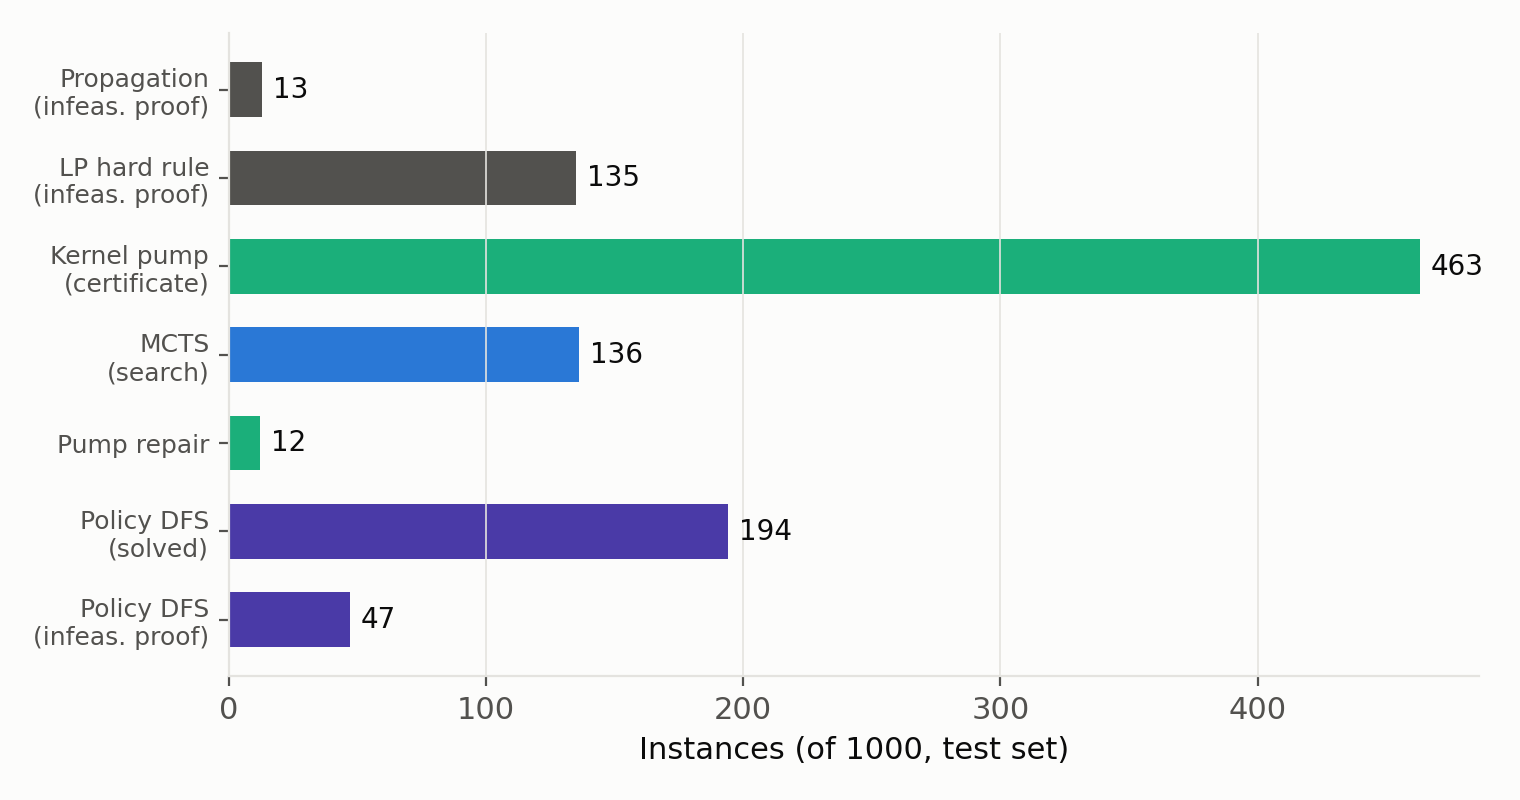
\includegraphics[width=0.85\textwidth]{v5_method_breakdown.png}
\caption{Decision-stage attribution over the 1{,}000 test instances.}
\label{fig:breakdown}
\end{figure}

\subsection{Ablation within the pipeline}

The DFS stage accounts for the decisive margin: without it, the pipeline scores 94.80\% / 76.12\% (feasibility / solution), which is at parity with LP rounding on feasibility while $+17.4$ points ahead on solution accuracy. The feasibility head contributed no correct rejections at any calibrated threshold; every gain in feasibility accuracy beyond the LP hard rule came from proofs (propagation, pump certificates implying feasibility, DFS exhaustion). This is an honest negative result for the learned feasibility head at this instance size and a target for the next iteration.

\section{Insights and Limitations}

\paragraph{Null-space structure is the workhorse.} The kernel pump---a direct operationalization of the project's null-space formulation---solves 57.9\% of feasible instances at negligible cost and never errs. The historical success of lattice reformulations on market-split systems \citep{aardal2000market} is thus mirrored inside a learned pipeline.

\paragraph{Proofs beat probabilities on this task.} The learned feasibility head, trained with a binary cross-entropy at the root, could not separate the hard LP-feasible-but-binary-infeasible instances (its probabilities cluster above 0.84 for both classes). Complete search under a learned ordering supplied the missing rejections as proofs. Learned components were most useful \emph{inside} the search (ordering, value estimation), consistent with the broader literature on learned branching \citep{gasse2019exact, nair2020solving}; end-to-end feasibility prediction appears harder in this regime even though message-passing networks have succeeded on satisfiability classification elsewhere \citep{selsam2019learning}.

\paragraph{Memorization on a fixed training pool.} Test solution accuracy peaked at epoch 10 and declined thereafter while training metrics improved, on a fixed pool of 10{,}000 instances replayed for 50 epochs. Periodic held-out evaluation and on-the-fly instance generation are recommended for the next training cycle.

\paragraph{Limitations.} (i) All results are at a single instance size ($10 \times 25$); size generalization---the project's central motivation---was deliberately deferred and remains unvalidated. (ii) Exact solvers dominate at this size; the pipeline's value proposition is prospective. (iii) The average inference time (1.03\,s) is dominated by MCTS on hard instances (std.\ 1.46\,s); the five residual false positives are budget artifacts, removable at higher DFS budgets at bounded extra cost. (iv) The training collapse at epoch 20, though transient, is unexplained and warrants investigation before longer runs.

\section{Conclusion}

A neuro-symbolic pipeline for binary linear systems was presented in which null-space projection, constraint propagation, MCTS with an AlphaZero-style policy target, and policy-guided complete backtracking are staged so that cheap certificates are attempted first and learned search is spent only on the hard residue. On the target distribution the pipeline exceeds the project's operational thresholds (feasibility $\geq$ 95\%, solution $\geq$ 75\%) with 99.50\% and 99.62\% respectively, decisively outperforming all inexact baselines, while exact solvers remain superior at this instance size. The next iterations will target the feasibility head's discriminative failure, on-the-fly instance generation to curb memorization, and the deferred size-generalization study.

\begin{thebibliography}{9}
\bibitem[Aardal et al.(2000)]{aardal2000market}
Aardal, K., Bixby, R. E., Hurkens, C. A. J., Lenstra, A. K., \& Smeltink, J. W. (2000). Market split and basis reduction: Towards a solution of the Cornu\'ejols--Dawande instances. \emph{INFORMS Journal on Computing, 12}(3), 192--202.

\bibitem[Cornu\'ejols \& Dawande(1998)]{cornuejols1998market}
Cornu\'ejols, G., \& Dawande, M. (1998). A class of hard small 0--1 programs. In \emph{Integer Programming and Combinatorial Optimization} (pp. 284--293). Springer.

\bibitem[Gasse et al.(2019)]{gasse2019exact}
Gasse, M., Ch\'etelat, D., Ferroni, N., Charlin, L., \& Lodi, A. (2019). Exact combinatorial optimization with graph convolutional neural networks. \emph{Advances in Neural Information Processing Systems, 32}.

\bibitem[Nair et al.(2020)]{nair2020solving}
Nair, V., Bartunov, S., Gimeno, F., von Glehn, I., Lichocki, P., Lobov, I., \ldots{} \& Zwols, Y. (2020). Solving mixed integer programs using neural networks. \emph{arXiv preprint arXiv:2012.13349}.

\bibitem[Selsam et al.(2019)]{selsam2019learning}
Selsam, D., Lamm, M., B\"unz, B., Liang, P., de Moura, L., \& Dill, D. L. (2019). Learning a SAT solver from single-bit supervision. \emph{International Conference on Learning Representations}.
\end{thebibliography}

\end{document}
